\documentclass[a4paper,12pt]{article}
\usepackage[utf8]{inputenc}
\usepackage[cm]{fullpage}
\usepackage{hyperref}
\usepackage[pdftex]{graphicx}
\usepackage{indentfirst}
\frenchspacing

\usepackage{amsmath}


\author{Lénárd Lajos Szánthó}
\title{Computer Simulations in Physics 1st Project:\\ Simulating the fruiting body formation\\ of Dictyostelium slime mould\\ and its fractal properties}


\begin{document}

\maketitle

\section{Motivation}

Dictyostelium is a genus of slime moulds originally thought to be fungi, but in the 20th century phylogenetic analysis has shown \cite{baldauf1997} that they are a sister-clade to fungi and animals as depicted on Figure \ref{fig:dictyophylo}. This revelation places them even earlier on the dated phylogenetic tree of life, which means that  -- among many other species -- they are around the transition from unicellularity to multicellularity. Multicellularity emerged multiple times independently along the tree of life, yet alone on the tree of fungi (\cite{nagy2018}) so identifying the phylogenetic relationships among and biological functions of these ''transition'' species  is one of the main goals of Biology today.

\begin{figure}
\centering
 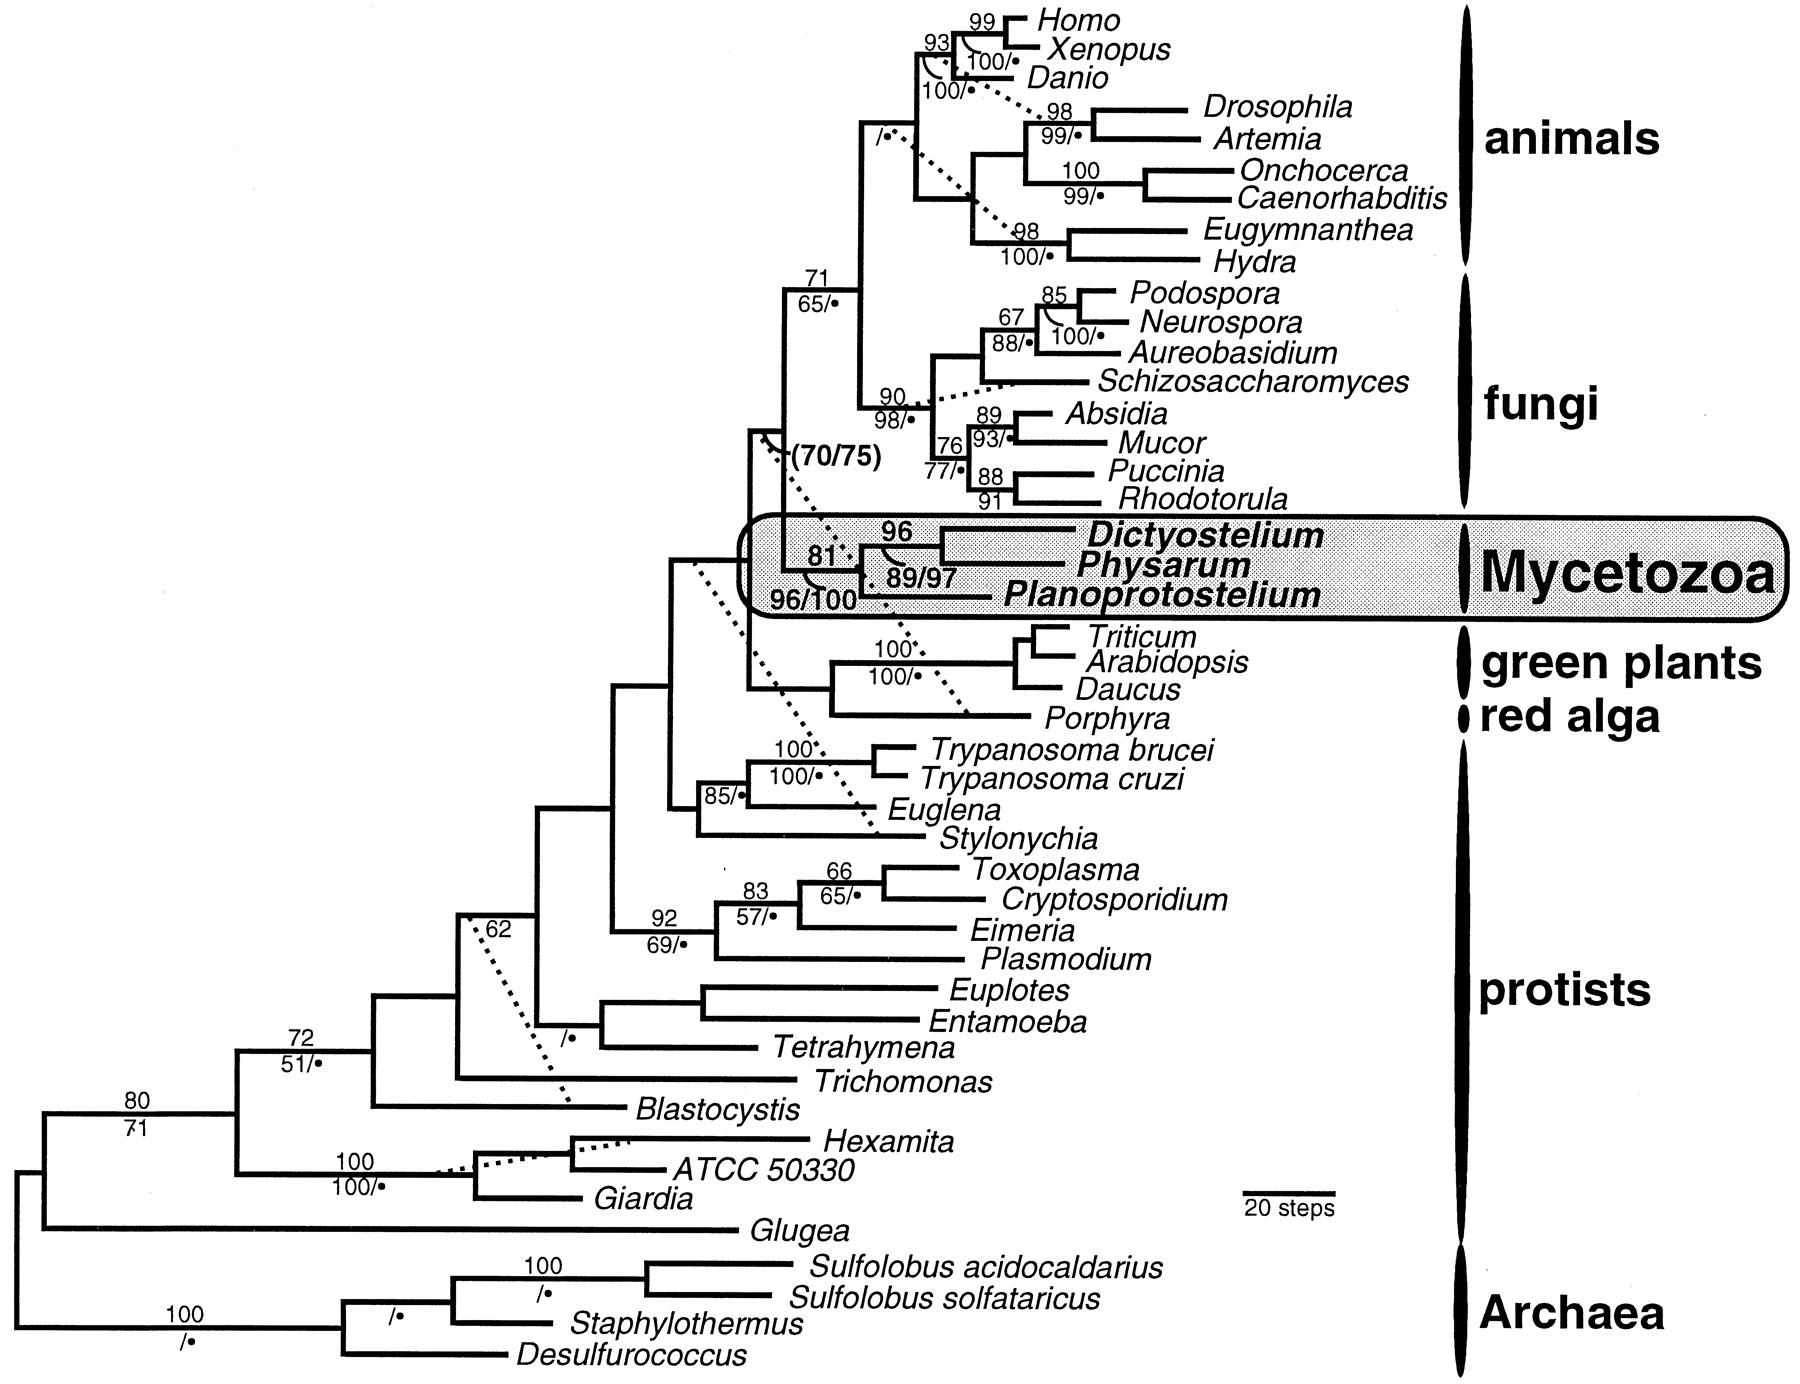
\includegraphics[width=\textwidth]{dictyophylo.jpg}
 \caption{Phylogenetic reconstruction of \cite{baldauf1997} showing that EF-1$\alpha$ amino acid sequences support a monophyletic, late-branching Mycetozoa}
 \label{fig:dictyophylo}
\end{figure}

The article \cite{kessler1993} -- whose simulation I am reproducing here -- catches one of the aspects of these questions: how do the unicellular Dictyostelium cells show multicellular pattern when their food source is depleted? Keep on reading to explore the remarkable process, how Dictyostelium cells work together and sacrifice themselves to build their fruiting body!

\section{Introduction}

Dictyostelium is an unicellular eukaryotic organism feeding on bacteria. Once the food source is depleted it releases a chemical signal, cyclic adenosine monophosphate (cAMP) which -- once reached a threshold concentration -- switches the cells into multicellular-like behaviour: they start to aggregate and then exit the 2D space and build a fruiting body which can be carried away by wind or animals to a new feeding ground where their offsprings can prosper again. Some Dyctiostelium individuals are sacrificed in the process which is yet another typical trait of multicellularity.

The aggregation pattern can be observed visually and MacKay \cite{mackay1978} decided to write a simulation with the goal of quantifying the process. I base my simulation on another paper by Kessler and Levine \cite{kessler1993} which introduces the problem in a more formal yet compact way.

They base their simulation on an extended diffusion equation:
\begin{equation}
\label{eq:egy}
 \frac{\partial c}{\partial t} = a^2 \nabla^2 c - \Gamma c + \textrm{sources}
\end{equation}
where $a$ is the lattice size, $\Gamma$ is the decay constant, and sources are continuously refreshed based on the position and state of the cells.

The cells themselves oblige to the following rules as described in \cite{kessler1993}:
\begin{itemize}
 \item a cell has three states: dormant, excited, recovery
 \item a dormant cell becomes excited if the cAMP concentration ($c$) is above threshold ($c_\text{threshold}$)
 \item an excited cell remains excited for $\tau$ time and releases $\Delta c$ cAMP in total during this period
 \item after $\tau$ long excitation the cell enters a $t_\text{R}$ time long recovery phase, during which it cannot be excited again
 \item when in excited state, the cell tries to move to a higher concentration neighbouring coordinate, if not already occupied
 \item only one successful move is allowed per excited state
\end{itemize}


\section{Writing the simulation}

The code for the simulation is published on GitHub\\ \url{https://github.com/drenal/dictyostelium-camp}, please read the commits, \emph{README.md} files and the code itself to have a full picture of the simulation and the obstacles met along the way. Below I just mention some of these in a dense format.  

The simulation can be started with different parameter settings which correspond to the model explained in the previous section:
\begin{itemize}
  \item -a LATTICE, --lattice LATTICE Lattice size ($a$)
  \item -g GAMMA, --gamma GAMMA decay constant ($\Gamma$)
  \item -r RHO, --rho RHO  density of cells ($\rho$)
  \item -c THRESHOLD, --threshold THRESHOLD Threshold concentration ($c_\text{threshold}$)
  \item -d CAMP, --camp CAMP  Amount of cAMP released by excited cell over period of tau ($\Delta c$)
  \item -t TAU, --tau TAU     Timespan of a cell being in excited state ($\tau$)
  \item -R RECOVERY, --recovery RECOVERY Timespan of a cell being resistant to excitation ($t_\text{R}$)
  \item -m MESH, --mesh MESH  1D size of the 2D mesh to simulate on (it's always a square mesh)
  \item -s STEPS, --steps STEPS Steps to run PDE for
  \item -i IMPORTSTATE, --import IMPORTSTATE Import state from base path's files
  \item -o OUTPUT, --output OUTPUT Output state files base name
  \item -S SAMPLING, --sampling SAMPLING Number of steps to sample after
\end{itemize}


I have decided to use Object Oriented Programming paradigm to write the simulation mixed with the efficiency of vectorized procedural methods. The former was used for the cells, the later for the PDE solver (which was wrapped in a class, but is not following any real OOP-pattern). Some time was spent deciding on the best way to incorporate global settings (like size of mesh, cellular properties, etc.) into the simulation, at first I preferred to have a singleton class to hold all these properties which would then shared among all the class instances of the simulation, but in the end I have decided to use Python's class properties feature, which was the simplest to implement, yet achieving the goal of not having too much redundant data stored in the memory and possibly leading to inconsistent settings during the simulation.

The logic to decide where the cell moves can be understood in two ways in the paper \cite{kessler1993}:
\begin{itemize}
 \item the cell tries to move to the maximum concentration neighbour and fails if it's occupied
 \item the cell tries to move to the maximum concentration neighbour which is empty
\end{itemize}

I have implemented the later one, so a list is created of the neighbours with higher concentration than at the current position of the cell, but this creates thick-branched aggregation, so maybe the authors used the former rule.

The simulation first had PDE-solver and plotting together but this led to very slow runtimes (4 hours and above) and also to the inflexibility of changing the plots or reanalysing the in-between results. 

I have killed two birds with one shot by orchestrating a state export mechanism which could be used both for creating the plots and for using them as inputs to continue the simulation from a given state. With this tweak the simulation time dropped from hours to minutes.

It was planned to also explore unit testing with Python in depth, but because of time constraints this was not done.

The Python module \emph{cProfile} was used to benchmark the code and find bottlenecks. It has shed light on many bugs too.

I have tried to make the cell's update mechanism multithreaded, but creating the threads and copying the results back and forth in the memory made it not worth it. The PDE obviously couldn't be parallelised.

Once the simulation was efficient and free of programming and logical errors (at least hopefully), the next task at hand was to find the right parameters for the diffusion equation coupled with a cell machine. For this purpose bash scripts were utilized with the GNU-tool \emph{parallel} to test many setups in a reasonable amount of time.

It turned out that the decay constant proposed by the \cite{kessler1993} paper ($\Gamma = 0.5$) was too strong, as shown on Figure \ref{fig:gammahalf}, one has to increase the cell density to 50\% so that signal transduction is not broken.

\begin{figure}
\centering
 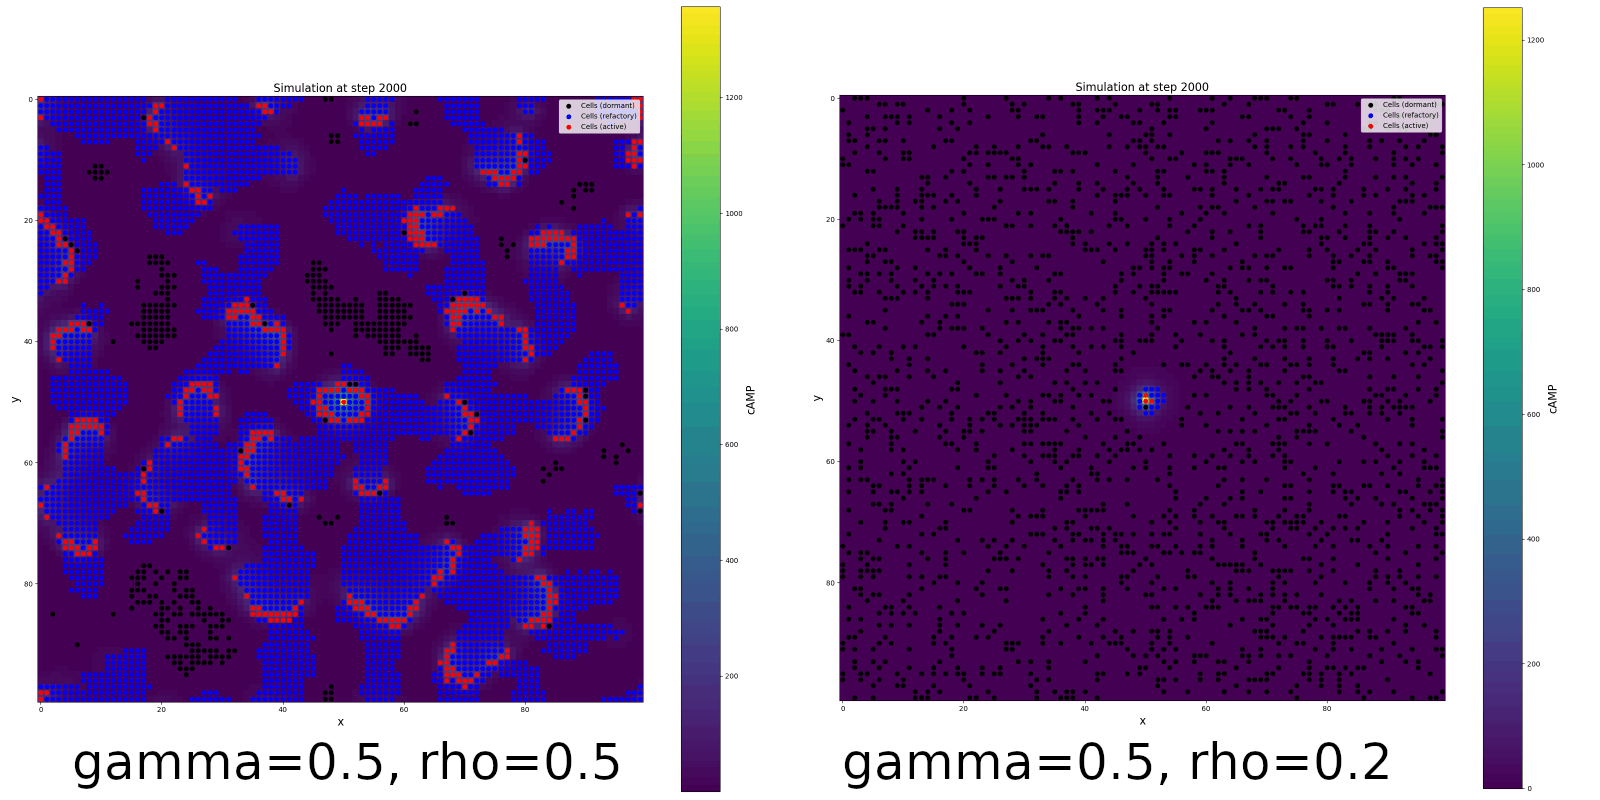
\includegraphics[width=\textwidth]{gammahalf.png}
 \caption{Final states of simulations started with the following parameters (on the left) $a=1$, $\Gamma=0.5$, $\rho=0.5$, $c_\text{threshold}=20$, $\Delta c=6000$, $\tau=2$, $t_\text{R}=20$ ; (on the right) $a=1$, $\Gamma=0.5$, $\rho=0.2$, $c_\text{threshold}=20$, $\Delta c=6000$, $\tau=2$, $t_\text{R}=20$. One can see that if the decay is too strong then a critical cell density (above 20\%) is needed for successful signal propagation. }
 \label{fig:gammahalf}
\end{figure}

I wanted to keep the 20\% cell density proposed by the paper, so I have explored the parameter space for $\Gamma$ and found that it should be lower than $0.13$ to get patterns similar to the observed aggregation of Dictyostelium. The other parameters (once $\Gamma$ and $\rho$ are fixed) have a stable range, then if changed the signal transduction gets broken fast or silent islands emerge, see e.g. Figure \ref{fig:tau} and Figure \ref{fig:recovery} where either the excitation time or the recovery time was changed from the ideal ($2$ and $20$) values.

\begin{figure}
\centering
 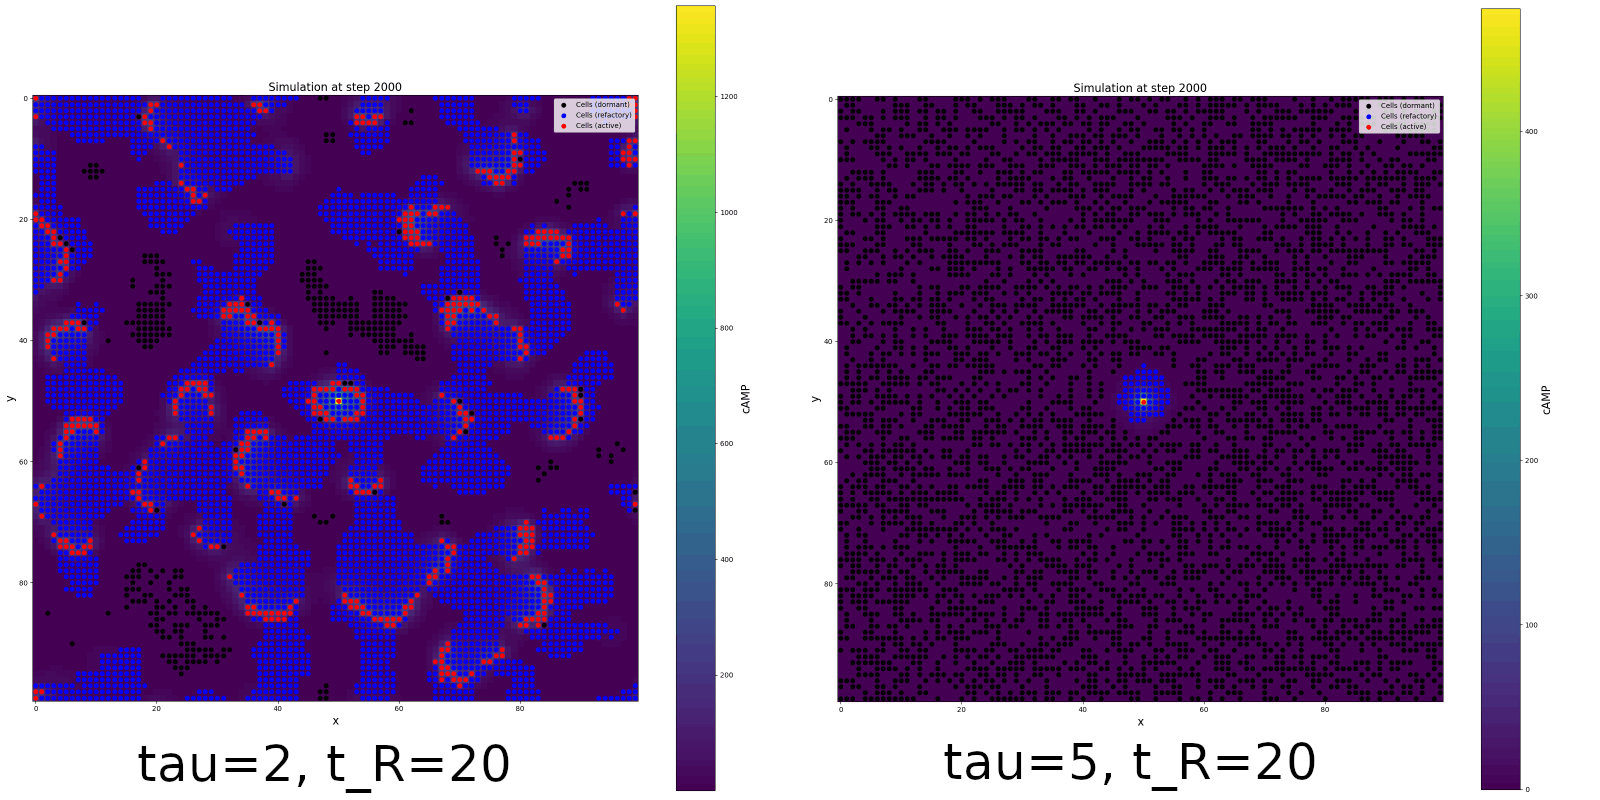
\includegraphics[width=\textwidth]{tau.png}
 \caption{Final states of simulations started with the following parameters (on the left) $a=1$, $\Gamma=0.5$, $\rho=0.5$, $c_\text{threshold}=20$, $\Delta c=6000$, $\tau=2$, $t_\text{R}=20$ ; (on the right) $a=1$, $\Gamma=0.5$, $\rho=0.5$, $c_\text{threshold}=20$, $\Delta c=6000$, $\tau=5$, $t_\text{R}=20$. One can see that if the cells spend more time active (which means more time to move), then the radius of signal transduction is very low (right picture).}
 \label{fig:tau}
\end{figure}

\begin{figure}
\centering
 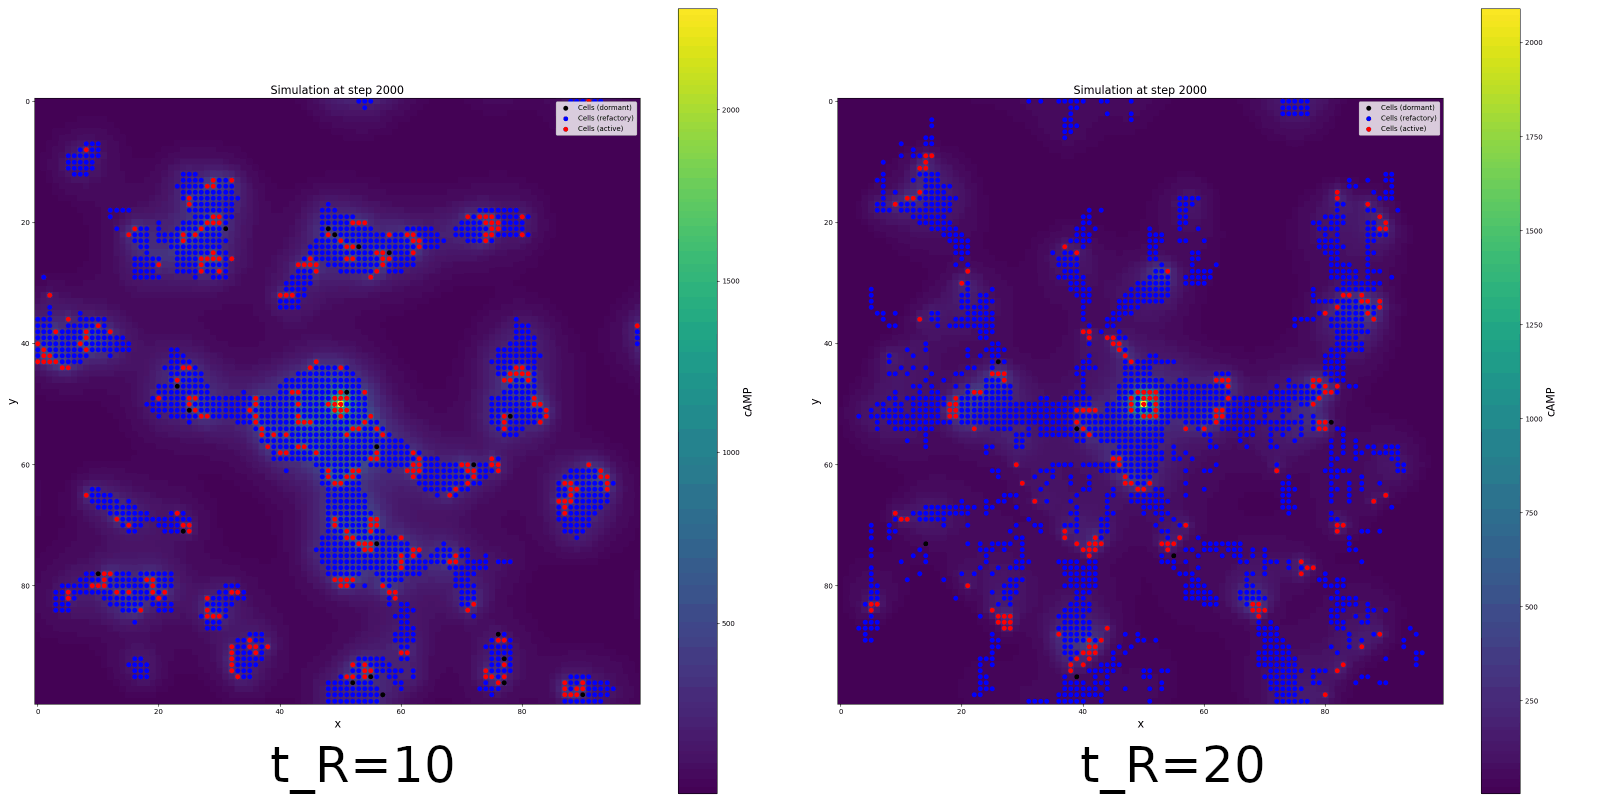
\includegraphics[width=\textwidth]{recovery.png}
 \caption{Final states of simulations started with the following parameters (on the left) $a=1$, $\Gamma=0.1$, $\rho=0.2$, $c_\text{threshold}=20$, $\Delta c=6000$, $\tau=2$, $t_\text{R}=10$ ; (on the right) $a=1$, $\Gamma=0.1$, $\rho=0.2$, $c_\text{threshold}=20$, $\Delta c=6000$, $\tau=2$, $t_\text{R}=20$. One can see that if the recovery time is shorter (cells get activated too soon compared to the concentration decay), we get thick branches.}
 \label{fig:recovery}
\end{figure}

After the parameter search was done and the best parameters are found the last step is to quantify the resulting patterns (see Figure \ref{fig:result}). For this I have chosen the fractal dimension which was determined with the box counting method. My code is heavily based on Dr Francesco's \cite{francesco2016} blog entry.

\begin{figure}
\centering
 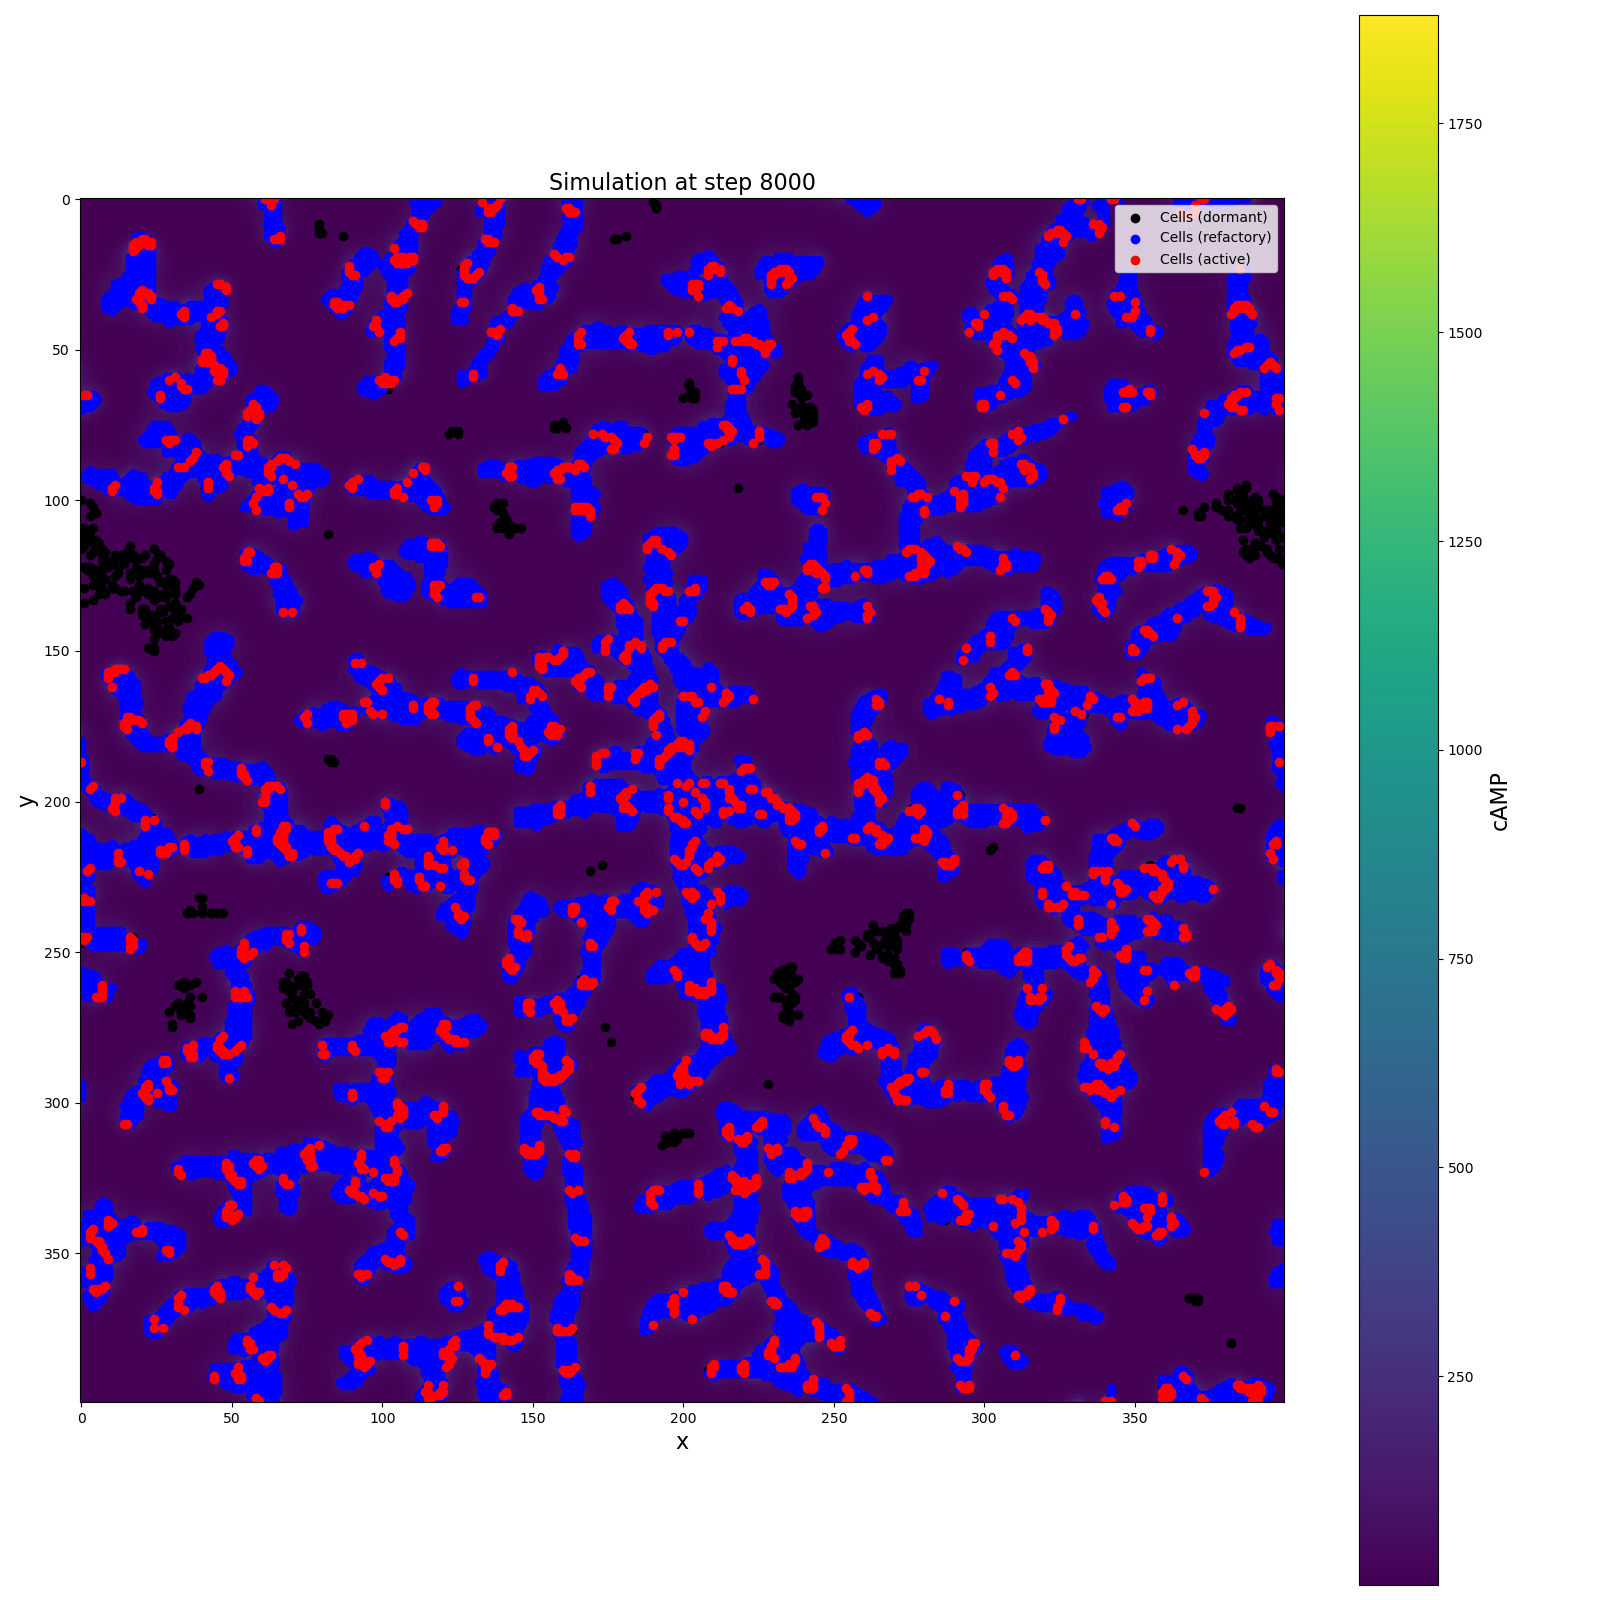
\includegraphics[width=\textwidth]{result.png}
 \caption{Final state of simulation started with the following parameters $a=1$, $\Gamma=0.115$, $\rho=0.2$, $c_\text{threshold}=20$, $\Delta c=6000$, $\tau=2$, $t_\text{R}=20$ with mesh size $400 \times 400$. Thin branches, periodic signal propagation through the whole population, yet not the anticipated fractal like structure.}
 \label{fig:result}
\end{figure}

The end results are the plots of the fitted lines on the box size versus number of needed boxes as shown on Figure \ref{fig:fractalfit}.

\begin{figure}
\centering
 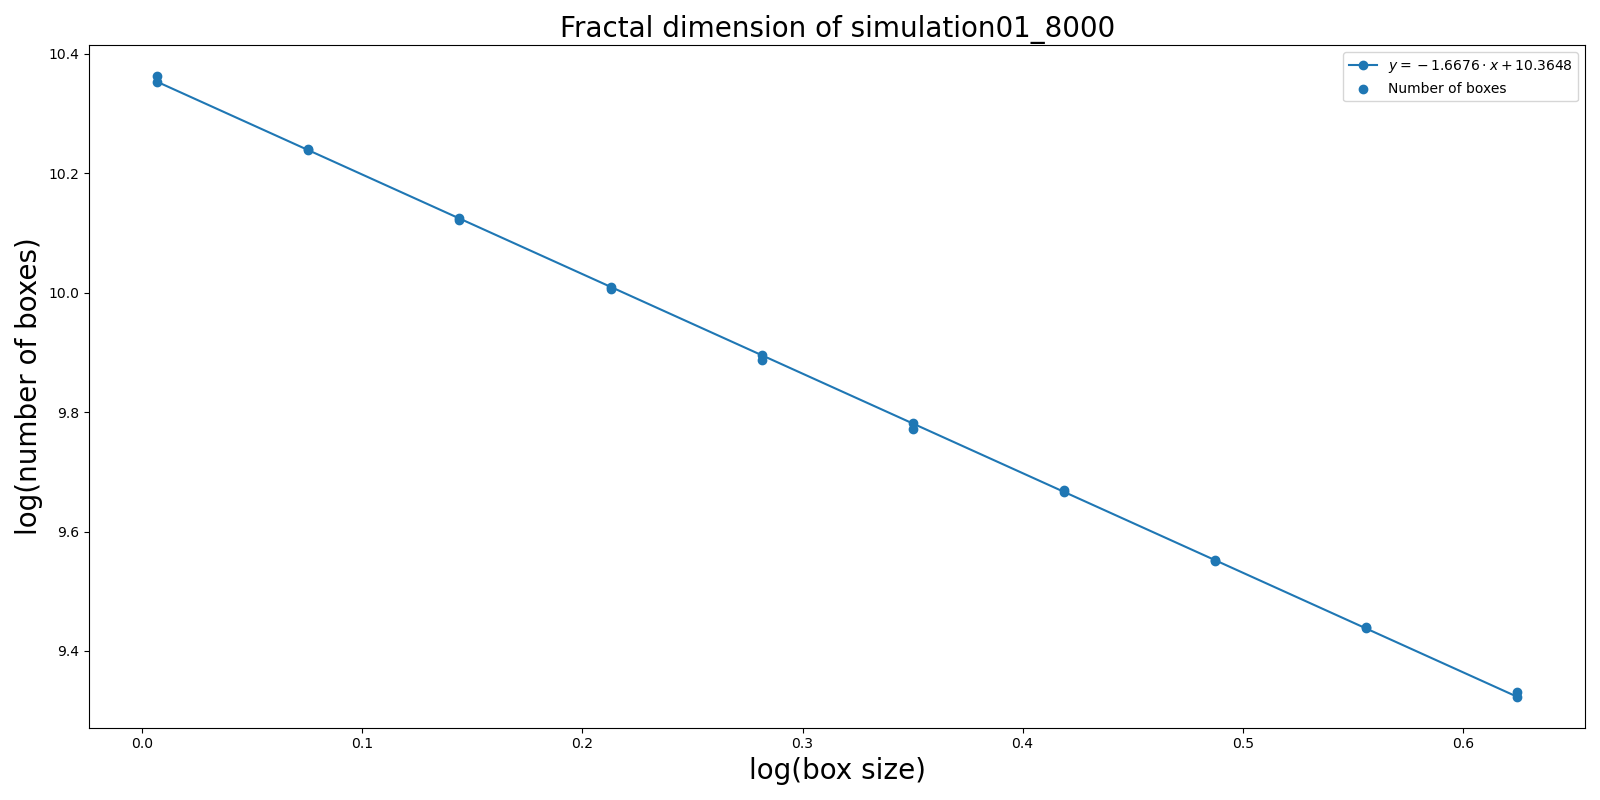
\includegraphics[width=\textwidth]{fractalfit.png}
 \caption{Fractal dimension fit result of the box counting method for the run presented on Figure \ref{fig:result}}
 \label{fig:fractalfit}
\end{figure}

\section{Discussion}

The goal of this project was to reproduce \cite{kessler1993} paper's results and quantify them with the help of fractal dimension. All the necessary tools were developed and tested in order to do so, yet the results are not as similar to the paper's as anticipated. Three obvious reasons can be accounted for this discrepancy: 
\begin{itemize}
 \item the aforementioned cell update logic which wasn't clear in the paper. Maybe they did not use the list of proposals to move to, which I decided to implement
 \item even with the extensive parameter space exploration maybe I did not find the best set of parameters to use
 \item the central source is an always-active, but paralyzed (cancerous) cell in my simulation. The paper \cite{kessler1993} mentions a periodic beacon or a spiral beacon.
\end{itemize}

Given enough time each of these possibilities could be explored and ruled out or proven.

The fractal dimension for 10 simulations with the best parameters $a=1$, $\Gamma=0.115$, $\rho=0.2$, $c_\text{threshold}=20$, $\Delta c=6000$, $\tau=2$, $t_\text{R}=20$ with mesh size $400 \times 400$ are:
\begin{equation}
 d = 1.6649 \pm 0.0229 \qquad (\delta=1.3\%)
\end{equation}

This means that the simulations are fairly stable against input parameters, no wild results, which would emerge from e.g. bugs in the code.

\section{Conclusion}

This project was full of fun, the goal to reproduce the results of a 1993 paper with a simple diffusion equation looked rather easy, I have underestimated the task's nuances, like the dependence on parameters (although it's still a fairly stable and predictable PDE-system), and its dependence on the chosen cell behaviour strategy. I also didn't expect to learn, that \emph{numpy}'s multiple dimensions array indexing is not as straightforward as one would think. 

I have made a simulation from scratch which implements a diffusion-equation solver with forward Euler method incorporating a layer of autonomous cells. The connection between the two systems is through the $\text{sources}$ term in the diffusion equation. During the project I have explored many \emph{Python}-specific best-practices and solutions (e.g. tricks to make a simulation faster), deepen my knowledge in numerical methods.

The results (e.g. Figure \ref{fig:pudgy}) although do not fully agree with the paper's \cite{kessler1993} results, this is probably due to the choice of cell movement strategy which was not clearly documented in the paper. It is interesting how we shifted in the last 2 decades to make the publications fully reproducible in many fields of science.

\begin{figure}
\centering
 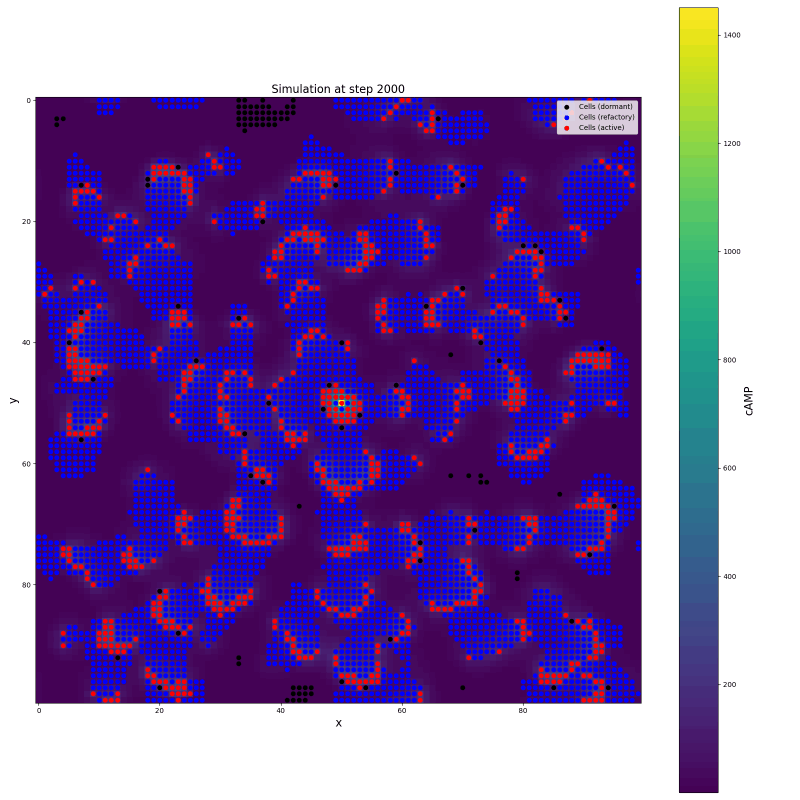
\includegraphics[width=\textwidth]{pudgy.png}
 \caption{Final state of simulation started with the following parameters $a=1$, $\Gamma=0.5$, $\rho=0.5$, $c_\text{threshold}=20$, $\Delta c=6000$, $\tau=2$, $t_\text{R}=10$ with mesh size $100 \times 100$}
 \label{fig:pudgy}
\end{figure}

\begin{thebibliography}{1}

\bibitem{kessler1993} David A. Kessler and Herbert Levine \emph{Pattern formation in Dictyostelium via the dynamics of cooperative biological entities} Physical Review E 48(\textbf{6}), 1993

\bibitem{baldauf1997} Sandra L. Baldauf and W. Ford Doolittle \emph{Origin and evolution of the slime molds (Mycetozoa)} PNAS 94 (\textbf{22}), 1997 \url{https://doi.org/10.1073/pnas.94.22.12007}

\bibitem{nagy2018} László G. Nagy, Gábor M. Kovács and Krisztina Krizsán \emph{Complex multicellularity in fungi: evolutionary convergence, single origin, or both?} Biol. Rev. pp. 000 – 000. 2018. \url{https://doi.org/10.1111/brv.12418}

\bibitem{landau2011} Rubin Landau, Manuel J. Paez and Cristian Bordeianu \emph{A Survey of Computational Physics: Python Multimodal eBook}. Princeton University Press, 2011

\bibitem{mackay1978} S.A. MacKay \emph{Computer simulation of aggregation in Dictyostelium discoideum} Journal of Cell Science 33: 1-16; 1978 \url{https://jcs.biologists.org/content/33/1/1}

\bibitem{francesco2016} Francesco Turci: \emph{Box Counting in Numpy}, 2016. Accessed: 2020-11-09 \url{https://francescoturci.net/2016/03/31/box-counting-in-numpy/}

\end{thebibliography}


\end{document}
